\section{Maximum Bipartite Matching} \index{bipartite graph} \index{maximum bipartite matching}

Given a \textit{\textbf{bipartite graph}} $G=(V,E)$ where $V = V_1 \cup V_2$ for some $V_1 \cap V_2 = \emptyset$ and $E \subseteq V_1 \times V_2$, a matching is a set of edges going from vertices in $V_1$ to vertices in $V_2$. The objective of the \textit{\textbf{maximum bipartite matching problem}} is to find a bipartite matching of the maximum cardinality.

There is a natural way to solve this problem using max flow. Given such bipartite graph, we can add a source node $s$ and target node $t$ and for all $u \in V_1$, add edge $(s,u)$ with capacity 1 and for all $v \in V_2$, add edge $(v,t)$ with capacity 1. Assign a capacity of 1 to all other edges already in $E$ (note that technically we need to turn those undirected edges into direct edges going from $V_1$ to $V_2$ but the construction for this is trivial so we won't spend time describing it formally).

\begin{figure}[htbp]
    \centering
    \includegraphics[width=0.7\linewidth]{maxflow/bipartite-matching.pdf}
    \caption{Maximum bipartite matching and its reduction to maximum flow problem.}
    \label{fig:maximum-bipartite-matching}
\end{figure}

Once we apply this construction to obtain a flow network, we can run any max-flow algorithms and the result gives rise to a matching with the maximum cardinality.

\begin{theorem}[Integrality Theorem] \index{integrality theorem}
    If the capacities in a flow network are integers, then the value of the maximum flow produced by the Ford-Fulkerson method is also an integer.
\end{theorem}

\begin{proof}
    By induction on the number of augmentations.
\end{proof}

Once we have the integrality theorem, we are able to prove the corrctness of the reduction from maximum bipartite matching to max flow. We do so by showing that there is an one-to-one correspondence between matchings of size $k$ in the original graph and flows of value $k$ in the flow network.

\begin{proof}
    \hfill

    (matching $\Rightarrow$ integral flow): Let $M = \{(u_1,v_1),\ldots,(u_k,v_k)\}$ be a matching of size $k$. We construct a flow $f$ such that for all $i = 1,\ldots,k$, $f(s,u_i) = f(u_i,v_i) = f(v_i,t) = 1$. It is easy to verify that $f$ is indeed a flow (by showing that it satisfies capacity constraint and flow conservation). The value of the flow $|f| = \sum_{v \in V}f(s,v) - \sum_{v \in V}(v,s) = k$.

    (integral flow $\Rightarrow$ matching): Let $f$ be a flow with value $k$. Let $M$ be the matching such that
    $$
    M = \{(u,v) \in E \mid u \in V_1,\,v \in V_2,\,f(u,v) = 1\}.
    $$
    Since a flow of $k$ comes out of $s$, there must be $k$ edges each with flow of 1 going from $s$ to distinct vertices in $V_1$. From each vertex in $V_1$, there must also be $k$ edges with flow 1 going into vertices in $V_2$ in order to satisfy the flow conservation property of a flow. Hence, $|M| = k$.
\end{proof}

\section{Hall's Theorem}

We now consider the problem of finding a perfect matching.

\begin{definition}[Perfect Matching] \index{perfect matching}
    A \textit{\textbf{perfect matching}} is a matching in which every vertex is matched. Let $G=(V,E)$ be an undirected graph with vertex partition $V = L \cup R$, where $|L|=|R|$. For any $X \subseteq V$, the neighborhood of $X$, denoted $N(X)$ is
    $$
    N(X) = \{y \in V \mid \text{$(x,y) \in E$ for some $x \in X$} \}
    $$
\end{definition}

The question is: when does a bipartite graph have a perfect matching. This is exactly what Hall's theorem answers. Hall's theorem establishes the necessary and sufficient condition for a perfect matching in bipartite graphs.

\begin{theorem}[Hall's Theorem] \index{Hall's theorem}
    Let $G$ be a bipartite graph where $V = V_1 \cup V_2$ and $V_1 \cap V_2 = \emptyset$. $G$ contains a perfect matching if and only if $|N(S)| \geq |S|$ for all $S \subseteq V_1$.
\end{theorem}

\begin{proof}
    By induction on the size of $V_1$.

    \textbf{Base case}: $|V_1| = 1$. The theorem trivially holds.

    \textbf{Inductive step}: Let $V_1$ be a set of vertices such that $|V_1|=k$ for some $k \geq 2$. Assume that for all vertex sets of size smaller than $k$, the theorem holds. Suppose bipartite graph $G = (V_1\cup V_2, E)$ satisfies Hall's condition.

    Case 1: For all $S \subsetneq V_1$, $|N(S)| \geq |S| + 1$. Let $(a,b)$ be an edge where $a \in V_1$ and $b \in V_2$. Let $G'$ be the subgraph induced by $V-\{a,b\}$. Clearly, $|V_1-\{a\}| \leq |N(V_1-\{a\})|$. Here's a more careful argument of why $G'$ satisfies Hall's condition. Let $S' \subseteq V_1-\{a\}$, and let $N'(S')$ denote the neighborhood of $S'$ in the graph $G'$ induced by $V-\{a,b\}$. Further, $S' \subseteq V_1-\{a\} \subset V_1$, so by assumption that $G$ satisfies Hall's condition,
    $$
    |N(S')| - 1 \geq |S'|
    $$
    Since only $b$ has been removed from the induced subgraph $G'$, we also have $|N'(S')| \geq |N(S')|-1$. It follows that $|N'(S')| \geq |S'|$ and Hall's condition holds for $G'$.
    
    By inductive hypothesis, $G'$ contains a perfect matching $M'$. Since $(a,b)$ connects $a \in V_1$ with $b \in V_2$, $\{(a,b)\}$ is a perfect matching. Hence, $M = M' \cup \{(a,b)\}$ is a perfect matching in $G$.

    \begin{figure}[htbp]
        \centering
        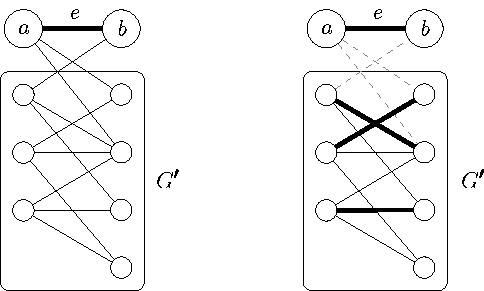
\includegraphics[width=0.5\linewidth]{maxflow/halls-thm-case1.pdf}
        \caption{Case 1. Note that $N(S')$ can have one fewer vertex than $N'(S')$ (this happens when there is an edge from some vertex in $S'$ to $b$, shown as dashed lines). $N(S')$ can also have the same number of vertices as $N'(S')$ if there is no edge going from vertices in $S'$ to $b$. Hence the inequality $|N'(S')| \geq |N(S')|-1$ holds. }
        \label{fig:halls-thm-case1}
    \end{figure}

    Case 2: There exists some $S \subsetneq V_1$ such that $|S| = |N(S)|$. Since $S$ is a proper subset of $V_1$, $|S| < |V_1|$. Let $G_1$ be the subgraph induced by $S \cup N(S)$. $S$ is a proper subset of $V_1$, and $V_1$ satisfies Hall's condition. It follows that any subset of $S$ must also be a subset of $V_1$ and hence satisfies Hall's hypothesis. By induction hypothesis, $G_1$ has a perfect matching $M_1$.

    \begin{figure}[htbp]
        \centering
        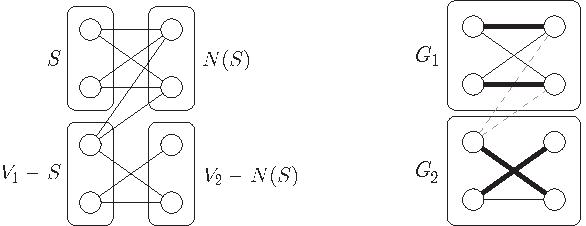
\includegraphics[width=0.6\linewidth]{maxflow/halls-thm-case2.pdf}
        \caption{Case 2. We partition $V_1$ into $S$ and $V_1-S$. The reasoning behind the construction $(S \cup S') \cup (N(S) \cup N(S'))$ when showing that $G_2$ satisfies Hall's condition is that there any neighboring vertices of $S'$ in $G$ not included in $N_{G_2}(S')$ should be included in $N(S)$, which allows us to derive a contradiction if $G_2$ does not satisfy Hall's condition.}
        \label{fig:halls-thm-case2}
    \end{figure}

    Let $G_2$ be the subgraph induced by $(V_1 - S) \cup (V_2 - N(S))$. We claim that $G_2$ also has a perfect matching. It suffices to show that $G_2$ satisfies Hall's condition. Suppose not, then there exists some $S' \subseteq (V_1-S)$ such that $|S'| > |N_{G_2}(S')|$ where $N_{G_2}(S')$ denotes the neighborhood of $S'$ in the subgraph $G_2$. More precisely, $N_{G_2}(S') = N(S) \cap (V_2-N(S))$. Consider the subgraph induced by $(S \cup S') \cup (N(S) \cup N(S'))$. Since $S \cup S'$ is a subset of $V_1$ and $G$ satisfies Hall's condition
    $$
    |N(S \cup S')| \geq |S \cup S'|
    $$
    Since $N(S)$ and $N_{G_2}(S')$ are disjoint,
    $$
    \begin{aligned}
        |N(S \cup S')| &= |N(S) \cup N_{G_2}(S')| \\
        &= |N(S)| + |N_{G_2}(S')| \\
        &= |S| + |N_{G_2}(S')| \\
        &< |S| + |S'| \\
        &= |S \cup S'|
    \end{aligned}
    $$
    which contradicts the assumption that $G$ satisfies Hall's condition. So, $G_2$ must also satisfy Hall's condition and by induction hypothesis, have a perfect matching $M_2$.

    $M_1$ and $M_2$ are perfect matchings within their individual subgraphs that are disjoint. Taking the union of $M_1$ and $M_2$ yields a perfect matching $M$ in $G$.

    By induction, Hall's theorem holds for bipartite graphs of all sizes.
\end{proof}

\section{Disjoint Paths} \index{disjoint path}

Given a graph (directed or undirected) $G=(V,E)$, two non-adjacent nodes $s$ and $t$, we say two paths $p$ and $p'$ from $s \leadsto t$ is are \textit{\textbf{edge-disjoint}} if the two paths do not share a common edge. The \textit{\textbf{maximum edge-disjoint paths}} problem wants to find the maximum number of edge-disjoint $s \to t$ paths. There is a simlilar but different notion of disjoint paths known as \textit{\textbf{interally disjoint paths}} or \textit{\textbf{vertex disjoint paths}} where instead of defining two paths $p$ and $p'$ as disjoint if they do not share an edge, we say two paths are disjoint only if they don't share a vertex. The problem of finding the maximum-size edge-disjoint paths is often useful in the context of communication networks, where we may want to evaluate the \textit{\textbf{fautlt tolerance}} of a network and ensure that there are sufficiently many edge-disjoint paths between two given nodes in the network.

\textit{\textbf{Menger's theorem}} states that the maximum number of edge-disjoint $s-t$ paths is equal to the minimum number of edges in an $s-t$ cut. We will present the theorem for both edge-disjoint paths and vertex disjoint paths. For the edge-based version, we will present an algorithm using max-flow to find the maximum number of edge-disjoint paths, and Menger's theorem follows immediately from the algorithmic construction and the max flow-min cut theorem.

For the vertex-based version, however, things are a little bit more complicated. It is easy to show the vertex-based version of Menger's theorem on a directed graph since we can follow the same construction as in the edge-based version. For undirected graphs, simply making every undirected edge a bidirectional directed edge is not enough, and we need some additional modifications to the original construction. We will also see another not quite constructive proof of Menger's theorem that does not directly rely on the max flow-min cut theorem.

\subsection{Edge-Disjoint Paths}

We first consider the problem of finding the maximum number of edge-disjoint paths on a directed graph. The construction is really simple. We simply take every edge in the graph and assign a capacity of 1. After this, we run compute the max flow on the graph, and the value of the final flow is the maximum number of edge-disjoint paths. This simple construction allows us to prove Menger's theorem for edge-disjoint paths.

\begin{theorem}[Menger's Theorem (edge)]
    Let $G=(V,E)$ be a graph and let $a,b \in V$ be two distinct vertices. The minimum number of \textbf{edges} in a $a,b$ separating cut equals the maximum number of \textbf{pairwise edge disjoint} $a \leadsto b$ paths in $G$.
\end{theorem}

\begin{proof}
    \hfill

    (edge-disjoint path $\Rightarrow$ flow): Let $\{p_1,\ldots,p_k\}$ be a set of $k$ edge disjoint paths from $s \leadsto t$. For all $e \in p$ for all $p \in \{p_1,\ldots,p_k\}$, let $f(e) = 1$. Since the paths are edge-disjoint, flow conservation and capacity constraints are clearly satisfied. Running the max flow algorithm on the flow network yields a flow with value of $k$.

    (flow $\Rightarrow$ edge-disjoint path): Let $f$ be a flow of value $k$. By construction of the flow network, there must be $k$ edges from $s$ with unit flow. For each edge $(s,u) \in E$, there must be an outgoing flow from $u$ in order to satisfy flow conservation. We can inductively build a path from $s$ to $t$ by picking an edge with unit flow. Repeat this for all $k$ outgoing edges from $s$, and we will have $k$ edge-disjoint paths.

    There is a one-to-one correspondence between the number of edge-disjoint paths and the value of the flow. It follows that when the value of the flow is maximized, we also have the maximum number of edge-disjoint paths. And by max flow-min cut, the value of the maximum flow is equal to the capacity of some $(S,T)$ cut. Since all edges have unit capacity, the number of edges separated by this cut is equal to the capacity of the cut. Therefore, the number of edges separated by this minimal cut is equal to the maximum number of edge-disjoint paths.
\end{proof}

\subsection{Vertex-Disjoint Paths}

Let $G=(V,E)$ be an undirected graph. We construct a directed graph $G'=(V',E')$ where:
\begin{itemize}
    \item[] $V' = \{s,t\} \cup \{v^-, v^+ \mid v \in V - \{s,t\}\}$ 
    
    \hfill

    \item[] $\begin{aligned}
        E' = &\{(s,v^-) \mid \{s,v\} \in E\} \cup \{(v^+,t) \mid \{v,t\} \in E\} \\
        &\cup \{(u^+,v^-) \mid \{u,v\} \in E\} \\
        &\cup \{(v^-,v^+) \mid v \in V\}
    \end{aligned}$
    
    \hfill
    
    \item[] $c(x,y) = \begin{cases}
        1 & \text{if $x=v^-$, $y=v^+$ for some $v \in V$ } \\
        \infty & \text{otherwise}
    \end{cases}$ 
\end{itemize}

Notice that every negative ($-$) vertex has exactly one outgoing edge connecting it to a positive ($+$) vertex. Conversely, every positive vertex has exactly one edge coming into it. Additionally, edges between negative and positive vertices have capacity of 1. This makes sure every internal vertex (that is not the source or sink) can only be visited once in the maximum flow.

\begin{figure}[htbp]
    \centering
    \includegraphics[width=0.9\linewidth]{maxflow/menger-undirected-construct.pdf}
    \caption{The construction converting an undirected graph to a directed graph when finding the maximum number of vertex disjoint paths on an undirected graph. The edges added between the vertices labeled $+$ and $-$ have capacity of 1, and were added to ensure every vertex can only be visited once because as soon as a vertex is visited, the edge become saturated and cannot admit more flow.}
    \label{fig:menger-undirected-construct}
\end{figure}

This construction converts an undirected graph into a directed graph, and we can prove Menger's theorem using an argument similar to how we proved it for the edge-based case.

\begin{theorem}[Menger's Theorem (vertex)] \index{Menger's theorem}
    Let $G=(V,E)$ be a graph and let $a,b \in V$ be two \textbf{non-adjacent} distinct vertices. The minimum number of \textbf{vertices} in a $a,b$ separating cut equals the maximum number of \textbf{internally vertex disjoint} $a \leadsto b$ paths in $G$.
\end{theorem}

\begin{proof}
    \hfill

    (flow $\Rightarrow$ vertex-disjoint path): Let $f$ be a maximum flow in the flow network constructed as shown above. For each negative vertex $v^- \in V'$, if there is a flow into $v^-$, then the value of the flow through $v^-$ must be 1 because $c(v^-,v^+)=1$. This flow must have originated from $s$ and arrived at $t$. Following this unit flow path gives us a path from $s$ to $t$. Since there are $|f|$ many unit flow paths from $s$ to $t$ and that the construction prevents a flow of value more than 1 through vertices other than $s$ and $t$, it follows that there are $|f|$ internally vertex disjoint $s \leadsto t$ paths in the original graph.

    (vertex-disjoint path $\Rightarrow$ flow): Let $(S,T)$ be a minimum cut with capacity $k$ in the flow network $G'$ constructed as shown above. We claim that every edge crossing the cut must be of the form $(v^-,v^+)$. Suppose not. Then, we must have an edge $(u,v)$ crossing the cut with infinite capacity. It follows that $c(S,T) = \infty$, which clearly contradicts the minimality of the cut. Finally, we show that the minimum cut $(S,T)$ corresponds to a cut in the original graph $G$. Let $U = \{u \in V \mid u^- \in S,\, u^+ \in T\}$. We have $|U| = c(S,T) = k$. Let $p = sv_1v_2\ldots v_t t$ be an undirected path from $s$ to $t$. We can construct an equivalent directed path $p' = s v_1^- v_1^+ v_2^- \ldots v_t^+ t$ in the flow network $G'$. The directed path $p'$ must contain an edge going from a negative vertex to a positive vertex, which are the edges crossing the cut $(S,T)$ by the claim proved earlier. Removing the edges crossing the cut disconnects $s$ from $t$ in $G'$. Then, by construction of $U$, removing vertices in $U$ will also disconnect $s$ from $t$ in $G$. Hence $U$ is a cut in $G$. Since $k$ is the capacity of the minimum cut, by max flow-min cut, we have $|U| = k = \text{max flow} = |f|$.
\end{proof}

\begin{figure}[htbp]
    \centering
    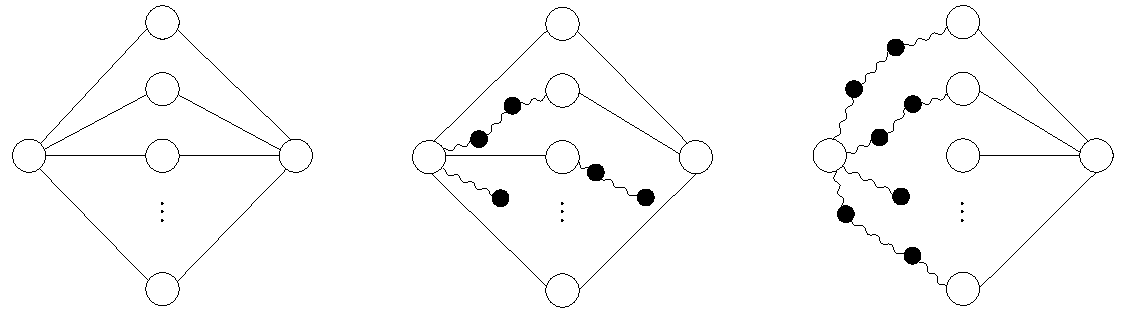
\includegraphics[width=0.9\linewidth]{maxflow/menger-1.pdf}
    \caption{The three possible cases in the inductive proof of Menger's theorem (vertex version). Straight lines indicate an edge connecting two vertices, and squiggly lines denote a path containing at least 3 vertices (including the initial and terminal vertices).}
    \label{fig:menger-undirected-1}
\end{figure}